\begin{figure}[!htbp]
\centering
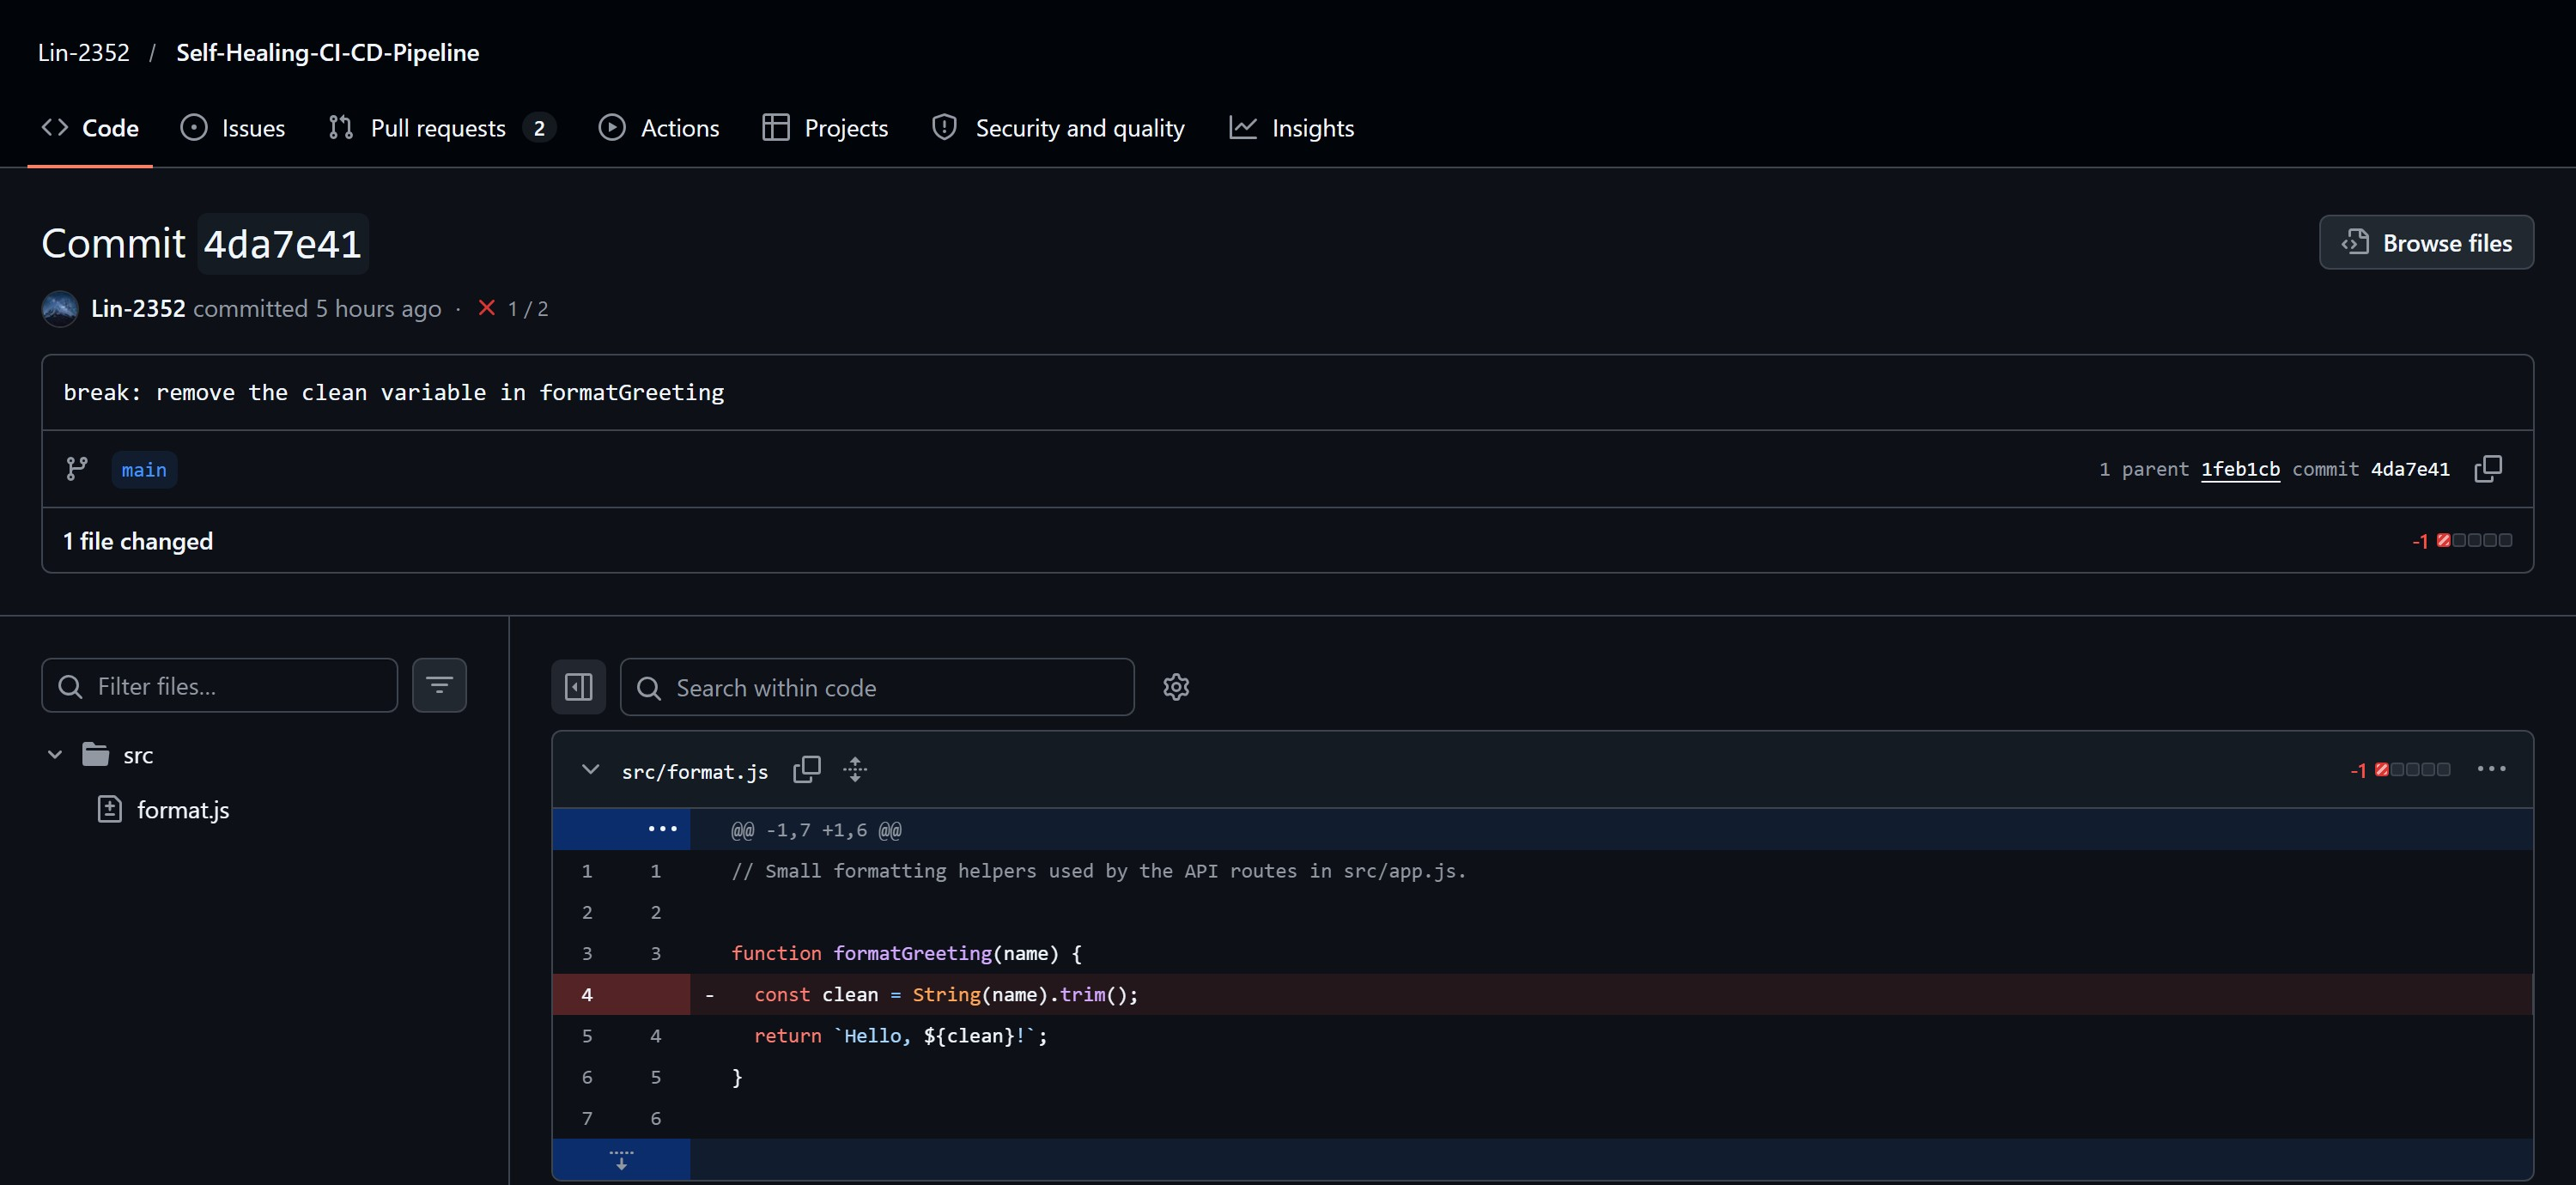
\includegraphics[width=\linewidth]{figures/shots/hq_commit.jpg}
\caption{The breaking commit \texttt{4da7e41}: one line is deleted from \texttt{src/format.js}.}
\label{fig:shot-commit}
\end{figure}
\begin{figure}[!htbp]
\centering
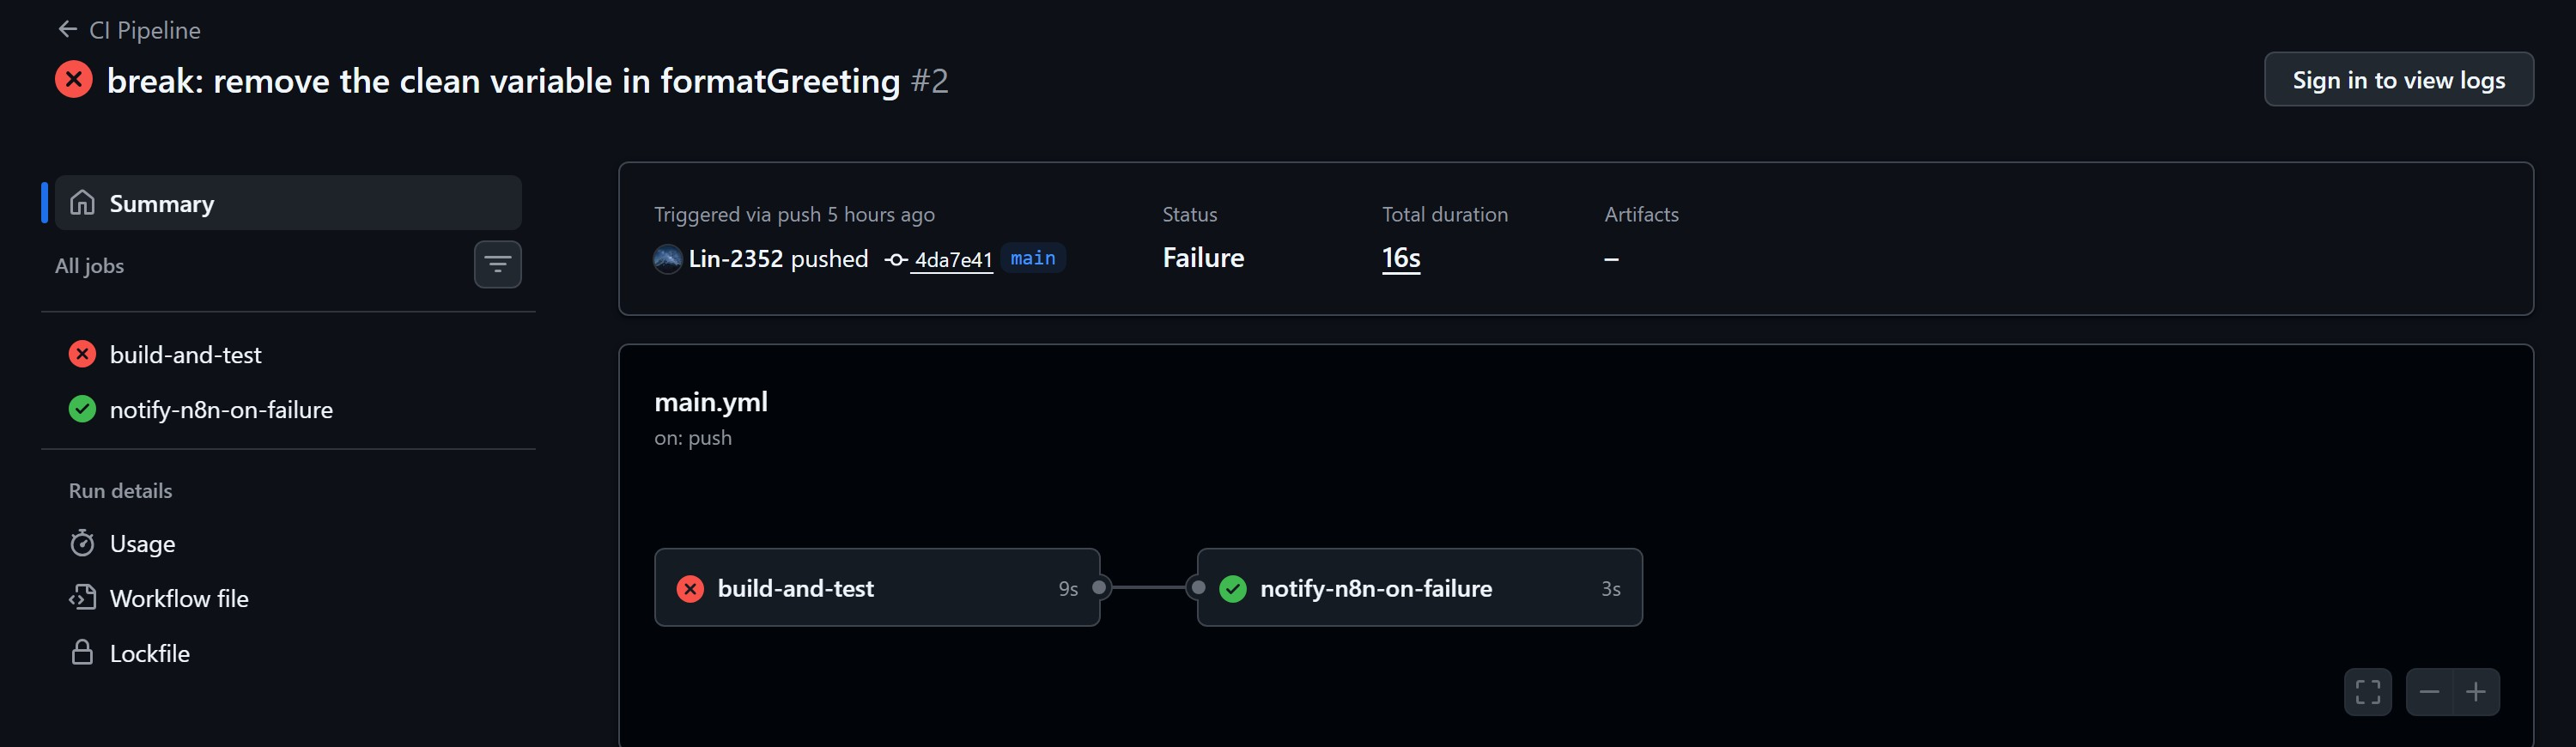
\includegraphics[width=\linewidth]{figures/shots/hq_run.jpg}
\caption{The failing run: \texttt{build-and-test} fails after 9 s, and the \texttt{notify} job that calls n8n passes.}
\label{fig:shot-failed-run}
\end{figure}
\begin{figure}[!htbp]
\centering
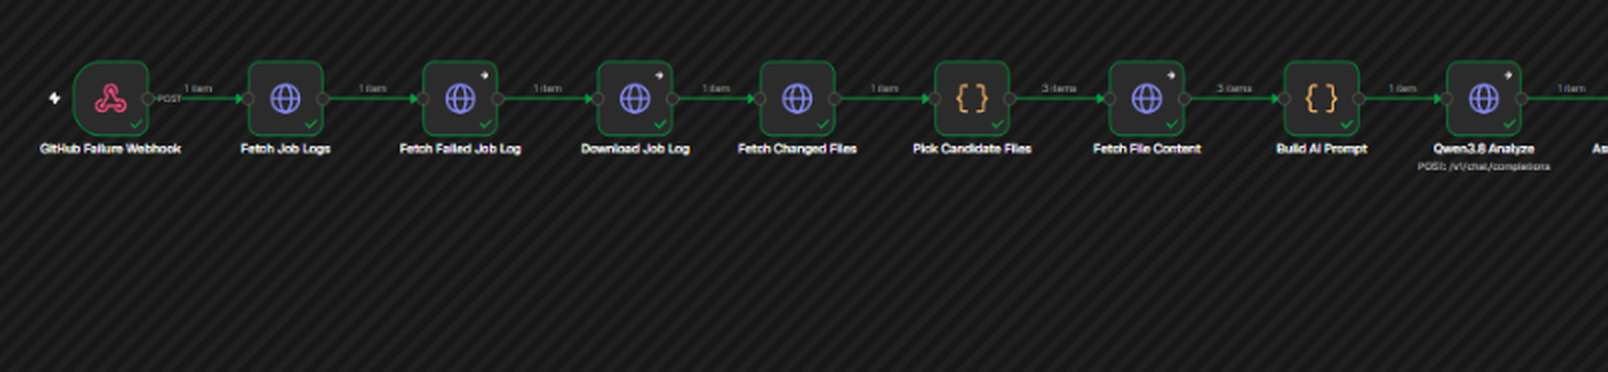
\includegraphics[width=\linewidth]{figures/shots/06a_n8n_left.png}\\[4pt]
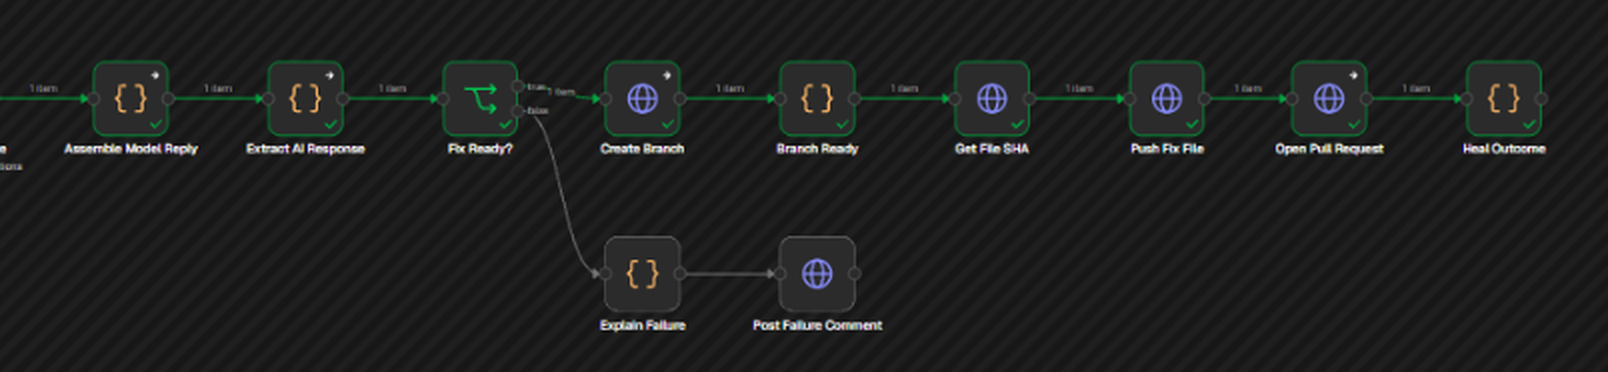
\includegraphics[width=\linewidth]{figures/shots/06b_n8n_right.png}
\caption{The n8n execution of the same run, shown in two halves: every node finished green in 18.7 s.}
\label{fig:shot-n8n}
\end{figure}
\begin{figure}[!htbp]
\centering
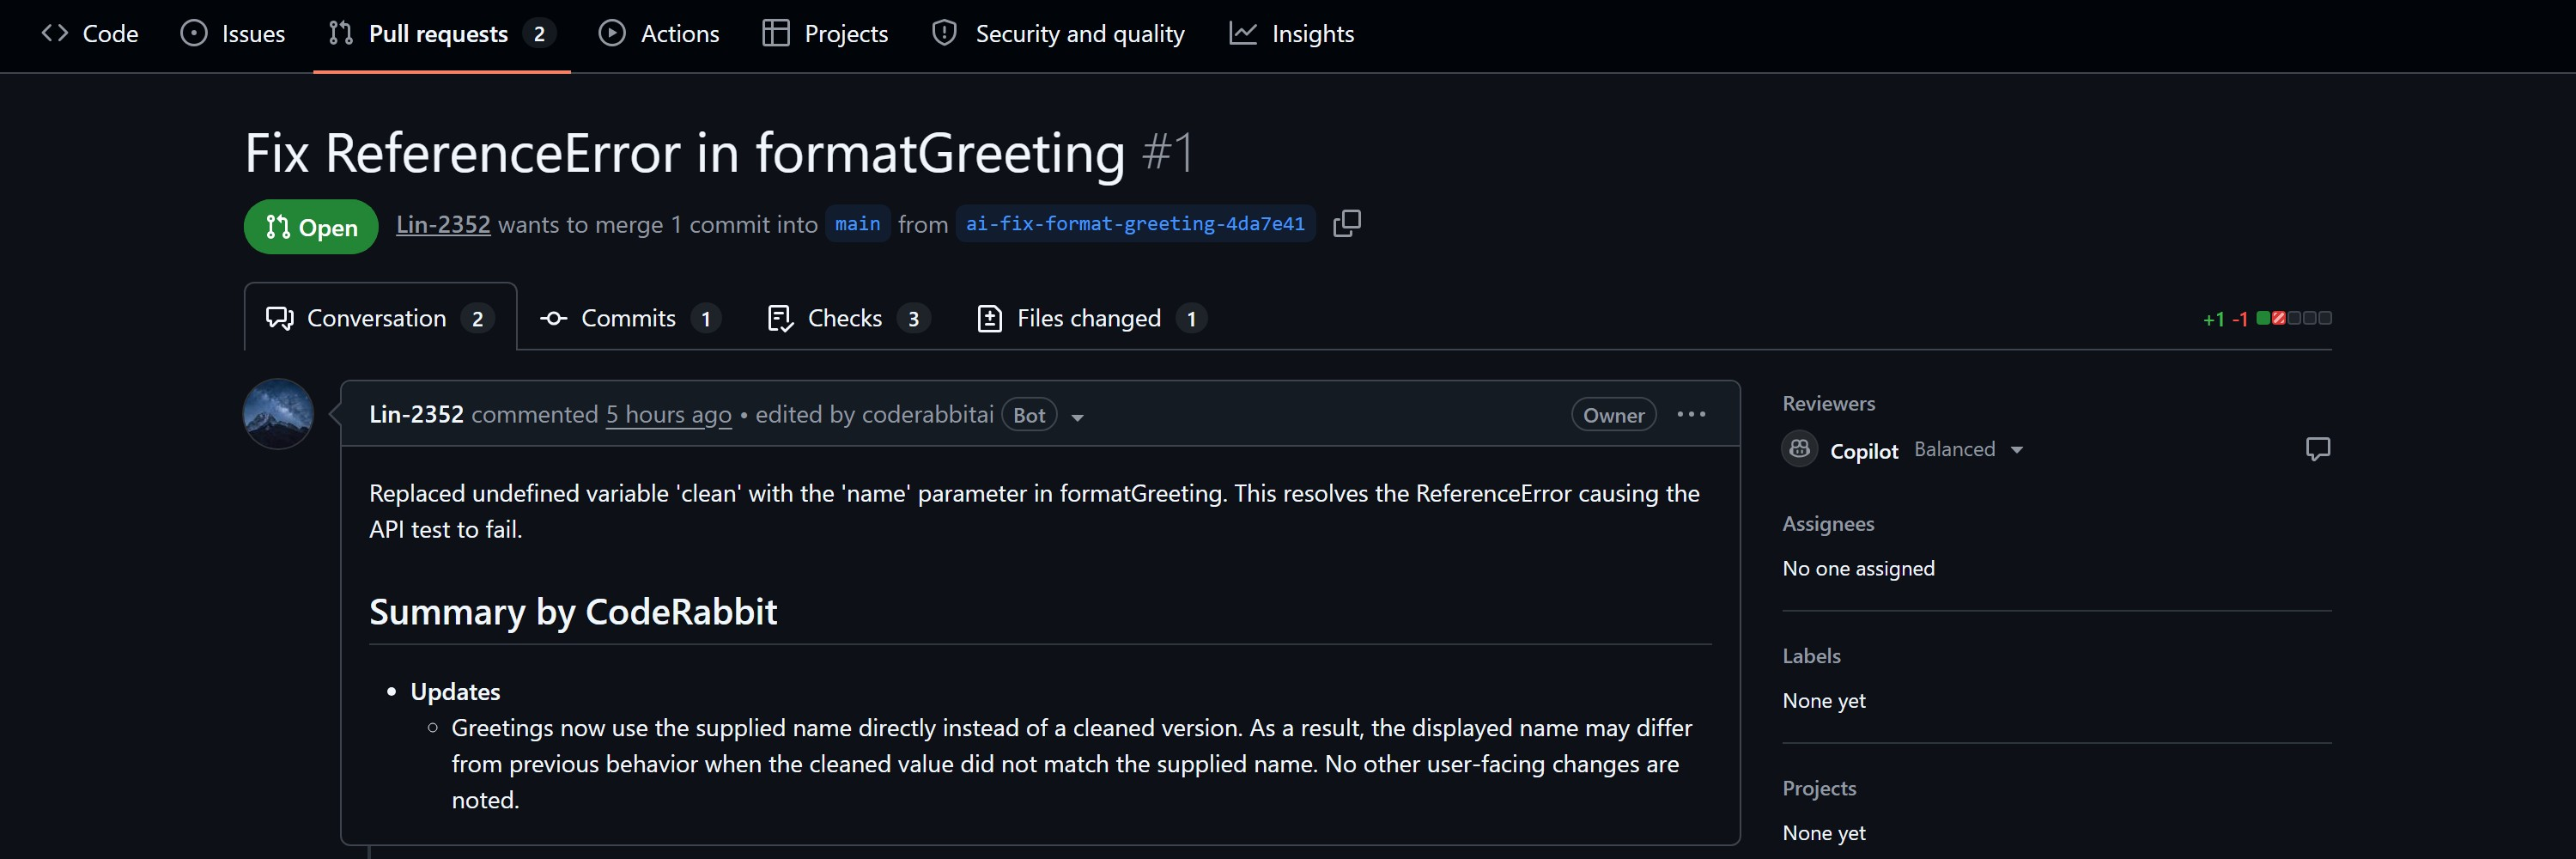
\includegraphics[width=\linewidth]{figures/shots/hq_pr.jpg}
\caption{The pull request opened by the workflow from the branch \texttt{ai-fix-format-greeting-4da7e41}.}
\label{fig:shot-pr}
\end{figure}
\begin{figure}[!htbp]
\centering
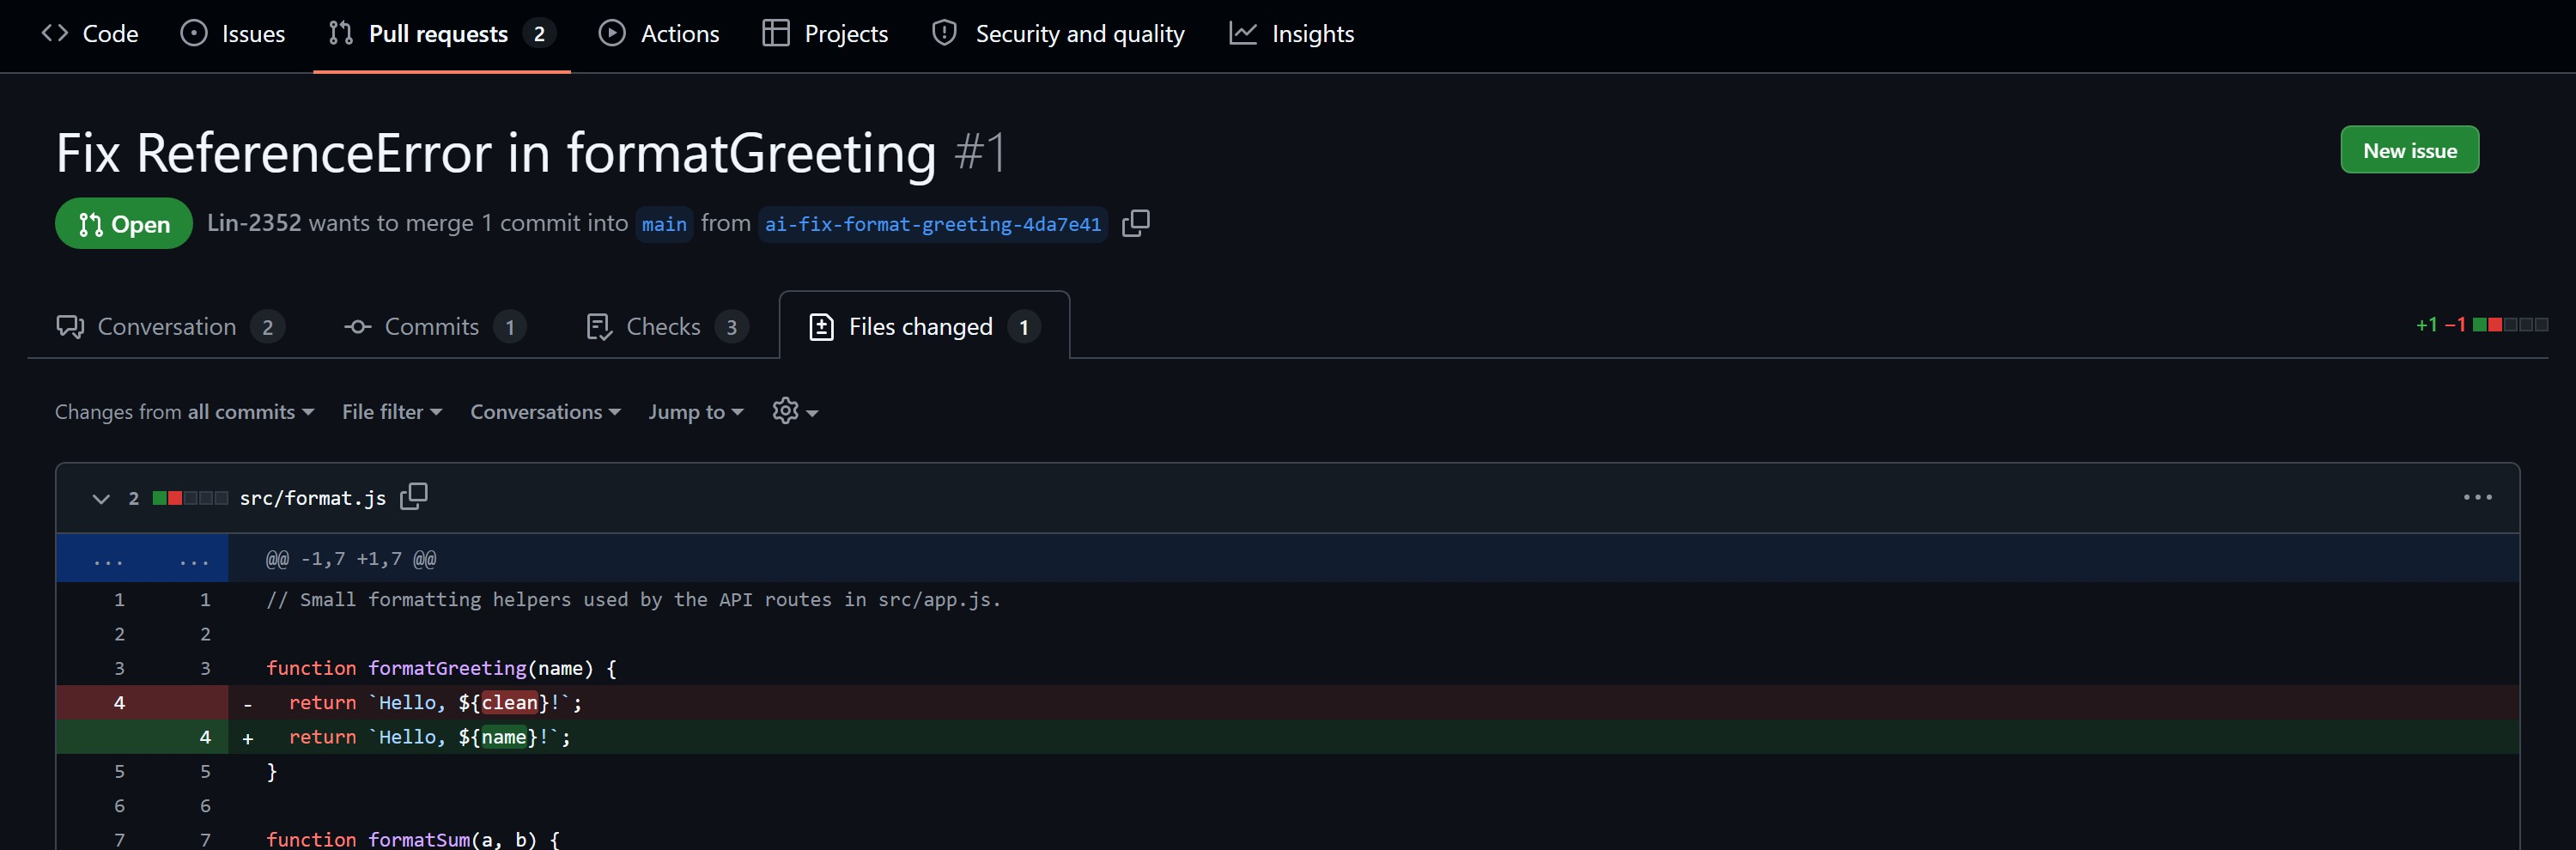
\includegraphics[width=\linewidth]{figures/shots/hq_pr_files.jpg}
\caption{The diff of the pull request: \texttt{\$\{clean\}} becomes \texttt{\$\{name\}}.}
\label{fig:shot-diff}
\end{figure}
\begin{figure}[!htbp]
\centering
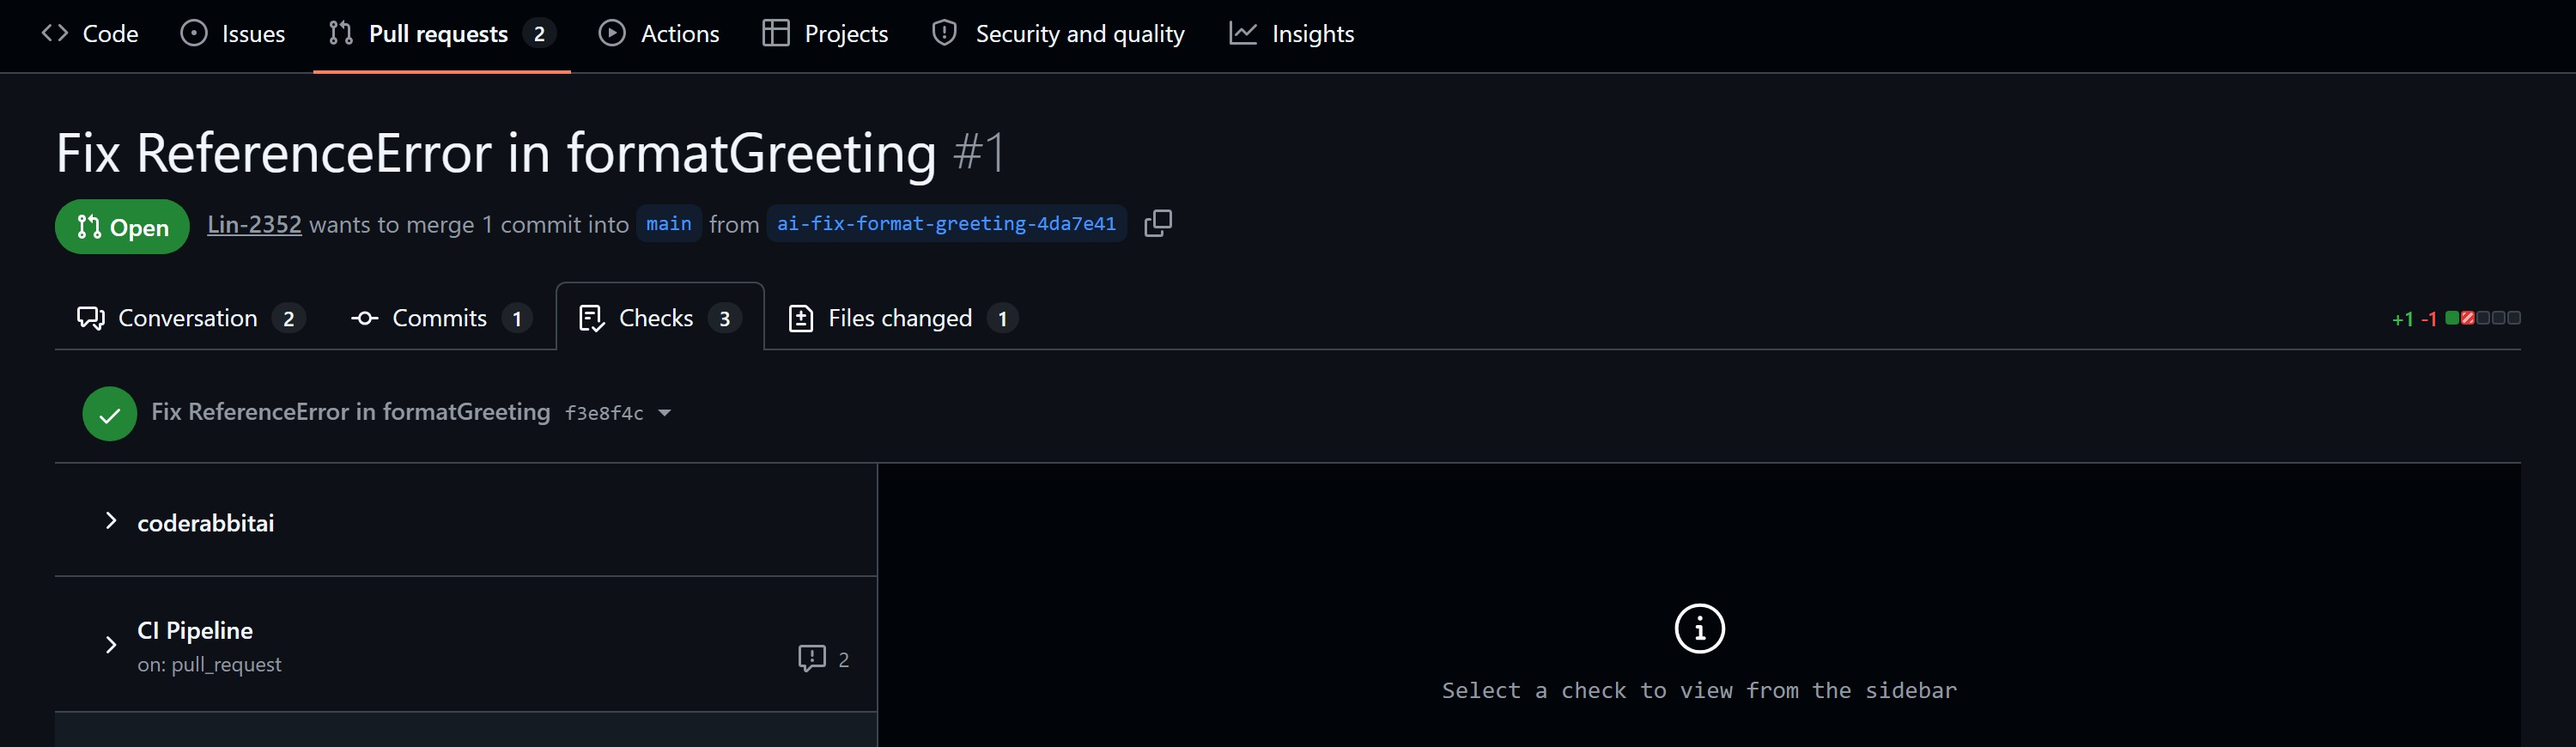
\includegraphics[width=\linewidth]{figures/shots/hq_pr_checks.jpg}
\caption{The checks of the pull request: CI on the fix passes.}
\label{fig:shot-checks}
\end{figure}
